%% Standalone figure: one pair of vectors described in two orthonormal bases.
%% Compile with pdflatex; QM.tex loads the resulting PDF with \includegraphics.
\documentclass[11pt]{standalone}   % Crops the page to the drawing; 11pt matches the notes
\usepackage{amsmath,amssymb}       % Math symbols
\usepackage{tikz}                  % Drawing
\usetikzlibrary{arrows.meta, calc} % Arrow tips; calc: orthogonal projection of a point onto a line

\begin{document}
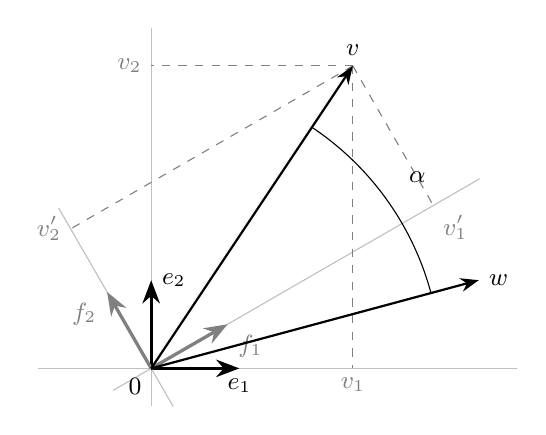
\begin{tikzpicture}[>=Stealth, scale=1.6, font=\small]
    \coordinate (O) at (0,0);
    % basis 1: e_1, e_2 along the axes
    \coordinate (E1) at (0.7,0);
    \coordinate (E2) at (0,0.7);
    % basis 2: f_1, f_2 rotated by 30 degrees
    \coordinate (F1) at (30:0.7);
    \coordinate (F2) at (120:0.7);
    % two vectors
    \coordinate (V) at (1.6,2.4);
    \coordinate (W) at (2.6,0.7);
    % lines along the basis directions
    \draw[gray!50] (-0.9,0) -- (2.9,0);
    \draw[gray!50] (0,-0.3) -- (0,2.7);
    \draw[gray!50] ($(O)!-0.5!(F1)$) -- ($(O)!4.3!(F1)$);
    \draw[gray!50] ($(O)!-0.5!(F2)$) -- ($(O)!2.1!(F2)$);
    % projections of v onto both bases
    \draw[dashed, gray] (V) -- ($(O)!(V)!(E1)$) node[below] {$v_1$};
    \draw[dashed, gray] (V) -- ($(O)!(V)!(E2)$) node[left] {$v_2$};
    \draw[dashed, gray] (V) -- ($(O)!(V)!(F1)$) node[below right] {$v_1'$};
    \draw[dashed, gray] (V) -- ($(O)!(V)!(F2)$) node[left] {$v_2'$};
    % basis vectors
    \draw[->, very thick] (O) -- (E1) node[below] {$e_1$};
    \draw[->, very thick] (O) -- (E2) node[right] {$e_2$};
    \draw[->, very thick, gray] (O) -- (F1) node[below right] {$f_1$};
    \draw[->, very thick, gray] (O) -- (F2) node[below left] {$f_2$};
    % the two vectors and the angle between them
    \draw[->, thick] (O) -- (V) node[above] {$v$};
    \draw[->, thick] (O) -- (W) node[right] {$w$};
    \draw ($(O)!2.3cm!(W)$) arc[start angle={atan(0.7/2.6)}, end angle={atan(2.4/1.6)}, radius=2.3cm];
    \node at ({(atan(0.7/2.6)+atan(2.4/1.6))/2}:2.6cm) {$\alpha$};
    \node[below left] at (O) {$0$};
\end{tikzpicture}
\end{document}